\documentclass[12pt,a4paper]{article}

\usepackage[left=2cm,right=2cm,top=2cm,bottom=2cm]{geometry} % less blank area
\usepackage{amsmath,amssymb,bm,dsfont} % for math
\usepackage{array}   % for eqnarray
\usepackage{arydshln}
\usepackage{graphicx}
\usepackage{enumerate} % for stylish enumrate
\usepackage{listings} % for code demonstration
\usepackage{color}    % for code highlight
\usepackage{fancyhdr} % for header and footnote
\usepackage{lastpage} % for calculating total pages
\usepackage{subfig} % for subfigure
\usepackage{tikz} % for drawing
\usepackage{pdfpages} % for importing PDF files

\newcommand{\docTitle}{IN2106 Practical Course -- Vision-based Navigation: Exercise \#2}
\newcommand{\docAuthor}{Min-An Chao (03681062)}
\newcommand{\docAuthorDept}{TUM MS Informatics}
\newcommand{\docAuthorEmail}{ga83fok@mytum.de}
\newcommand{\docDate}{29.04.2018}

\pagestyle{fancy}
\fancyhf{}
\lhead{\textit{\docTitle}}
\rhead{\textit{\docAuthor}}
\cfoot{\textit{- Page \thepage of \pageref{LastPage} -}}

\lstset{ language={},
         basicstyle=\ttfamily\footnotesize,
         keywordstyle=\color{blue}\ttfamily\footnotesize,
         commentstyle=\color{magenta}\ttfamily\footnotesize,
         morecomment=[l][\color{magenta}\footnotesize]{\#}
}

\setlength{\parindent}{0cm}
\setlength{\parskip}{0.5cm}

% for vector and matrix
\newcommand{\vct}[1]{\boldsymbol{#1}}
\newcommand{\mtx}[1]{\mathbf{#1}}
\newcommand{\set}[1]{\mathcal{#1}}
\newcommand{\dom}[1]{\mathbb{#1}}
\newcommand{\fnc}[1]{\text{#1}}

\DeclareMathOperator*{\argmin}{argmin}
\DeclareMathOperator*{\argmax}{argmax}

\begin{document}
    \title{\vspace{-1.75cm} \large \textsf{\textbf{\docTitle}}}
    \author{\normalsize \textsf{
        \textbf{\docAuthor} \hspace{6pt}\textbar\hspace{6pt}
        \docAuthorDept \hspace{6pt}\textbar\hspace{6pt}
        \docAuthorEmail}}
    \date{\small \textsf{\docDate}}
    \maketitle 
    \thispagestyle{fancy}
    \vspace{-0.5cm}
    \hrule

    \section{Left Jacobian in $SE(3)$}
   
    \textsf{\textbf{Proof}}
    From the Taylor's series we have,
    \begin{eqnarray}\label{eq:lj_proof}
      \sum_{n=0}^{\infty} \frac{1}{(n+1)!} (\vct{\phi}^{\wedge})^n
      &=& \sum_{n=0}^{\infty} \frac{1}{(n+1)!} (\theta \vct{a}^{\wedge})^n \nonumber\\
      &=& \underbrace{\mtx{I}}_{=\vct{a}\vct{a}^T - \vct{a}^{\wedge}\vct{a}^{\wedge}}
          + \theta \vct{a}^{\wedge} 
          + \frac{\theta^2}{2!}\vct{a}^{\wedge}\vct{a}^{\wedge} 
          + \frac{\theta^3}{3!}\underbrace{
            \vct{a}^{\wedge}\vct{a}^{\wedge}\vct{a}^{\wedge}
            }_{= -\vct{a}^{\wedge}}
          + \cdots \nonumber\\
      &=& \vct{a}\vct{a}^T
          + \underbrace{\left(  
            \theta - \frac{\theta^3}{3!} + \frac{\theta^5}{5!} - \cdots 
            \right)}_{= \sin \theta}
            \vct{a}^{\wedge}
          - \underbrace{\left(  
            1 - \frac{\theta^2}{2!} + \frac{\theta^4}{4!} - \cdots
            \right)  }_{= \cos \theta} 
            \vct{a}^{\wedge}\vct{a}^{\wedge}  \nonumber\\
      &=& \vct{a}\vct{a}^T
          + \sin \theta \vct{a}^{\wedge}
          - \cos \theta \underbrace{
            \vct{a}^{\wedge}\vct{a}^{\wedge}
            }_{ = \vct{a}\vct{a}^T - \mtx{I}}  \nonumber\\
      &=& \cos \theta \mtx{I}
          + (1 - \cos\theta) \vct{a}\vct{a}^T 
          + \sin \theta \vct{a}^{\wedge}.
    \end{eqnarray}
    
    \textsf{\textbf{Coding validation}}
    \begin{lstlisting}[frame=single,numbers=left]
given translation vector rho = (1 0 0)^T
given rotation matrix phi = 
      0.5 -0.866025         0
 0.866025       0.5         0
        0         0         1
from theta = 1.0472 and axis = (0 0 1)^T
SE3 xi = 
      0.5 -0.866025         0         1
 0.866025       0.5         0         0
        0         0         1         0
        0         0         0         1
se3 of xi = (   0.9069 -0.523599         0         0         0    1.0472)^T
its rotation matrix from exponent map = 
      0.5 -0.866025         0
 0.866025       0.5         0
        0         0         1
rotation matrix of Rodrigues' =
      0.5 -0.866025         0
 0.866025       0.5         0
        0         0         1
    \end{lstlisting}


    \section{Compare trajectories}
    \textsf{\textbf{Task 1}}
    The snapshot of plotting trajectories is shown in Fig.~\ref{fig:draw_trajectory},
    where red is for estimated trajectory and the blue the ground truth.
    \begin{figure}[!h]
        \centering
        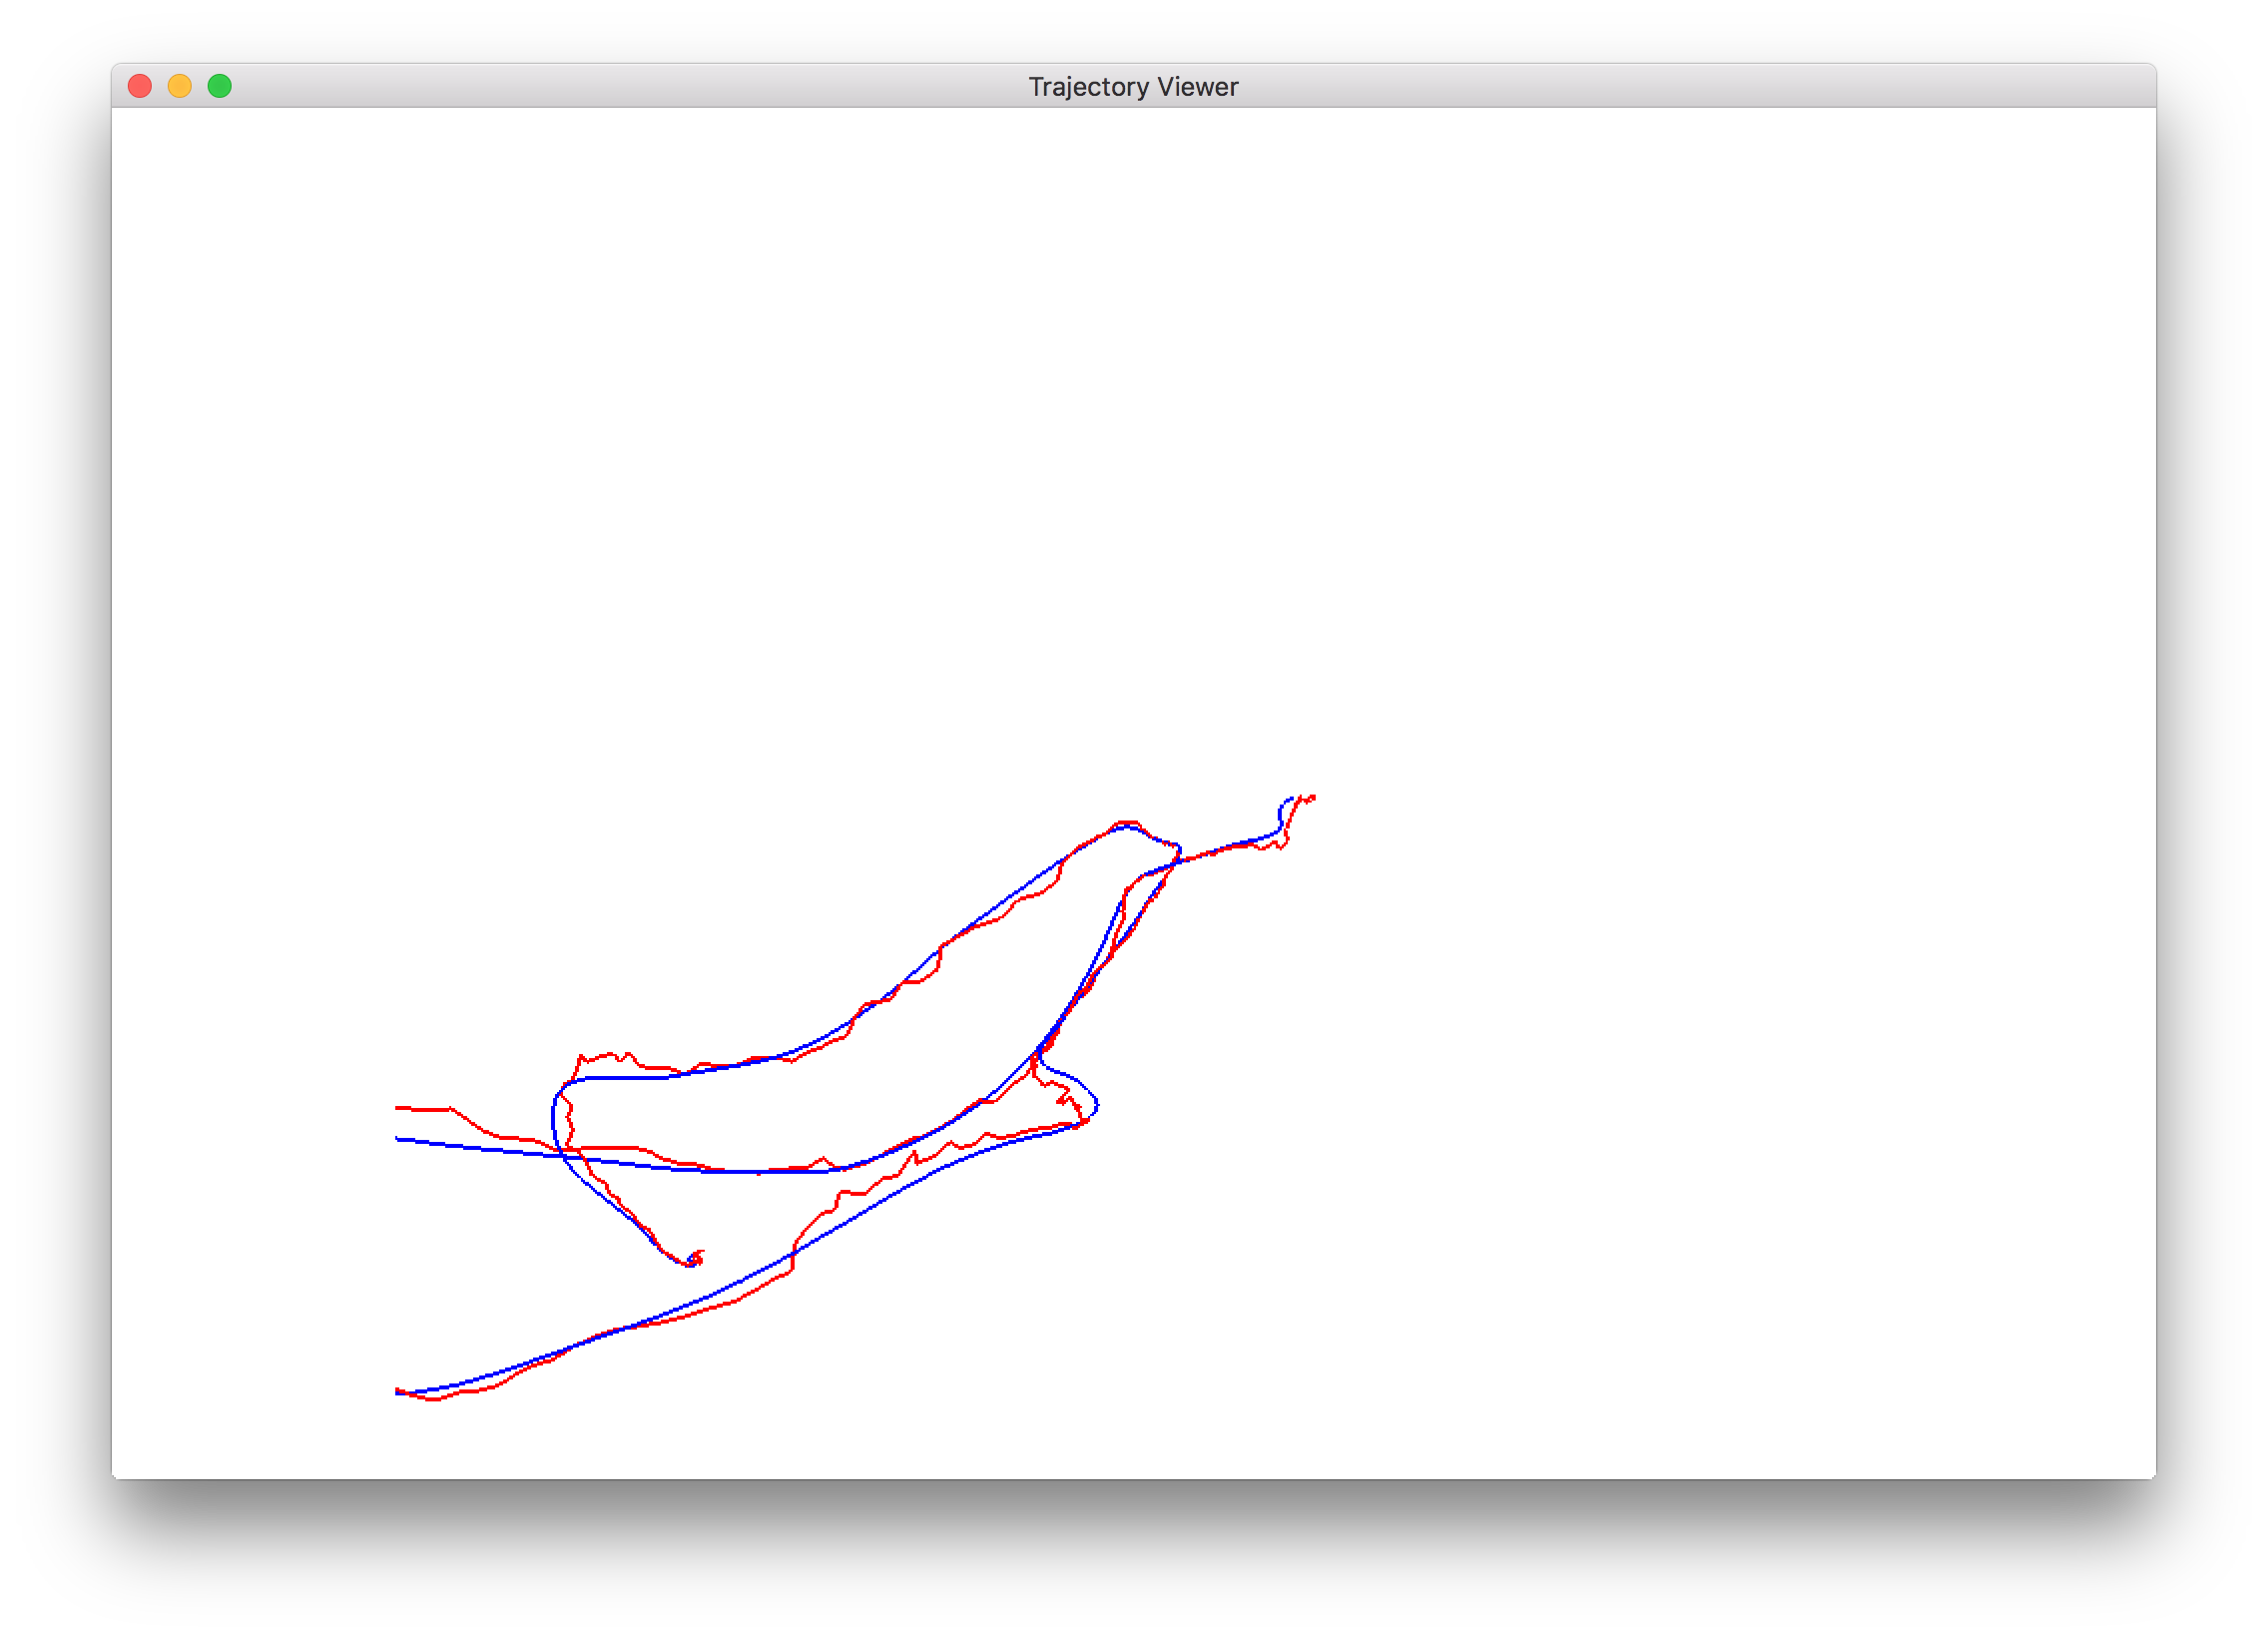
\includegraphics[height=6cm]{fig/draw_trajectory.png}
        \caption{Snapshot of \texttt{Pangolin} view of estimated trajectories and the ground truth}
        \label{fig:draw_trajectory}
    \end{figure}

    
    \section{Images, camera intrinsic and extrinsic}
    \textsf{\textbf{Task 1}}
    The recovered image is shown in Fig.~\ref{fig:undistort_image}.
    We can see now the straight line of windows and the edges of metal cylinders,
    which are distort in the original image.
    \begin{figure}[!h]
        \centering
        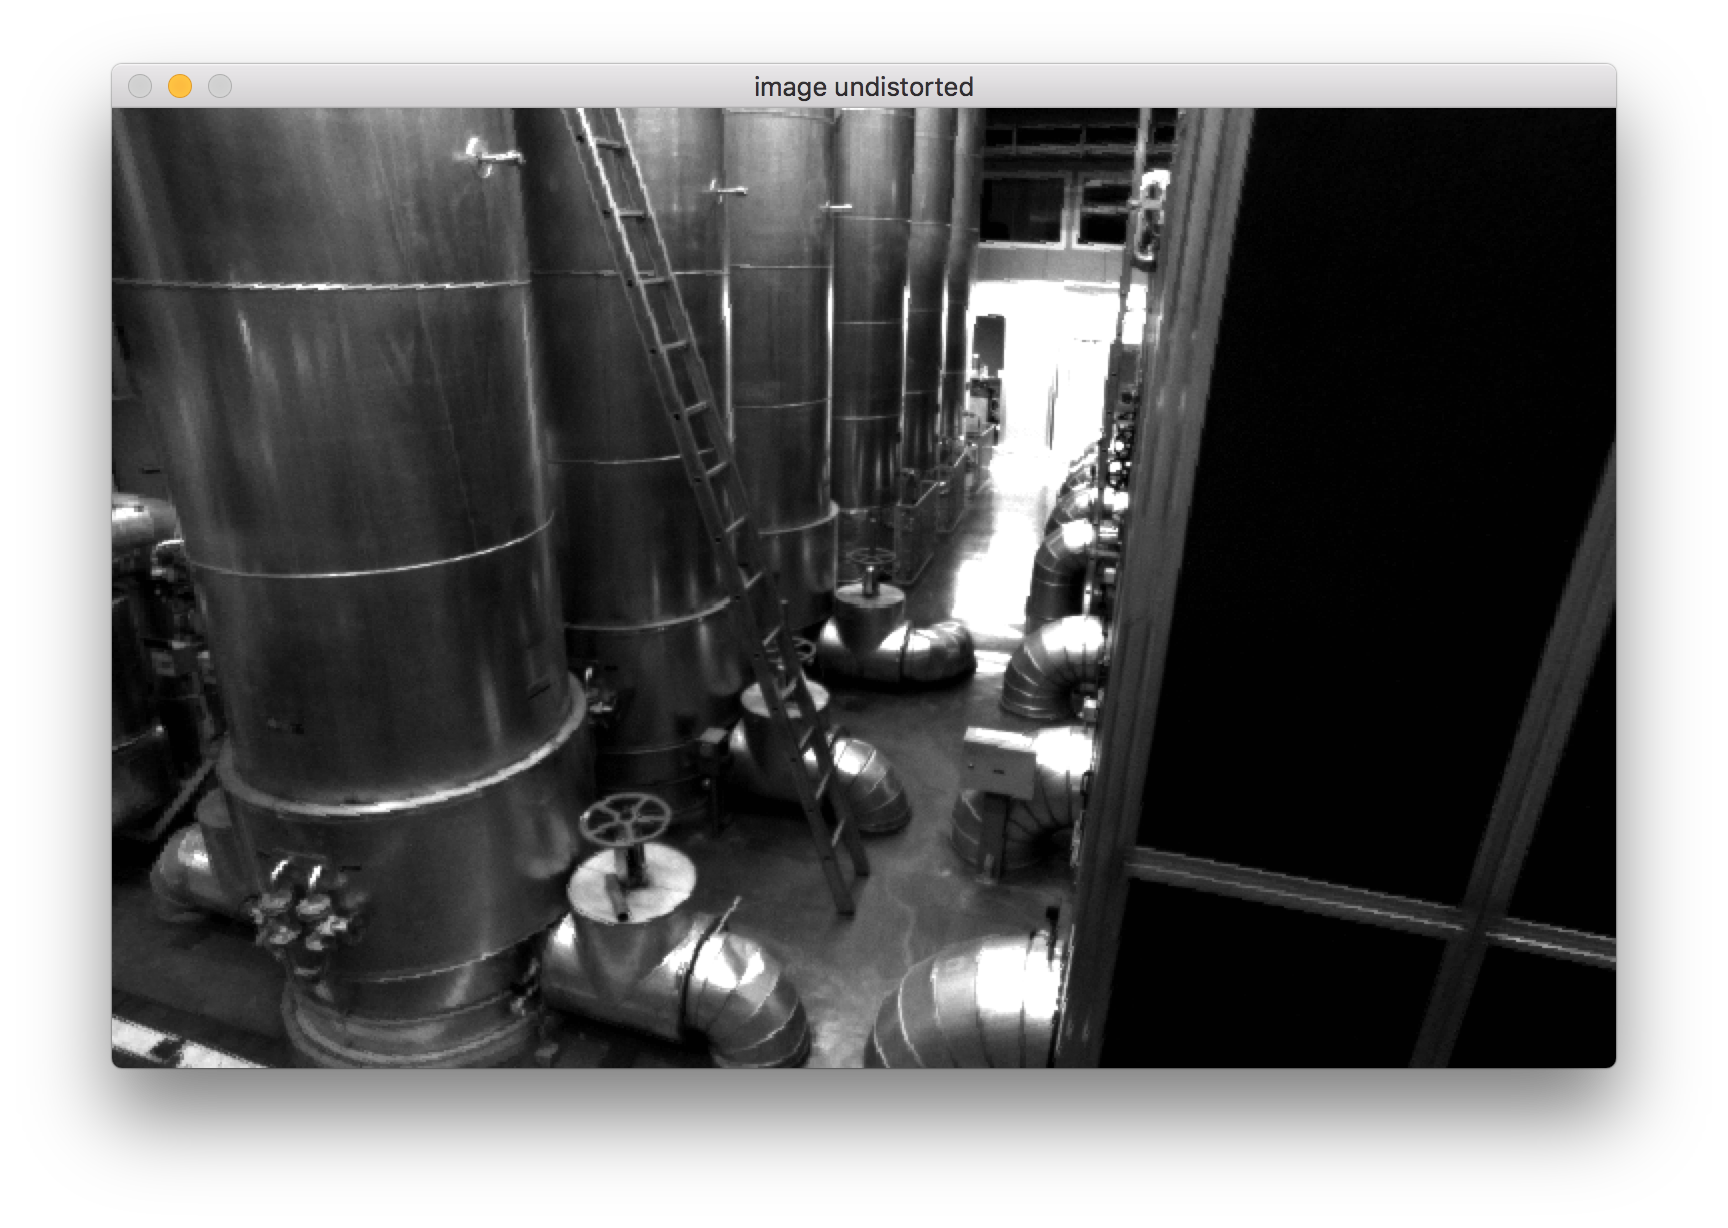
\includegraphics[height=6cm]{fig/undistort_image.png}
        \caption{Result of image undistortion}
        \label{fig:undistort_image}
    \end{figure}

    \textsf{\textbf{Task 2}}
    The snapshot of point cloud view of left-eye view is shown in Fig.~\ref{fig:disparity}.
    \begin{figure}[!h]
        \centering
        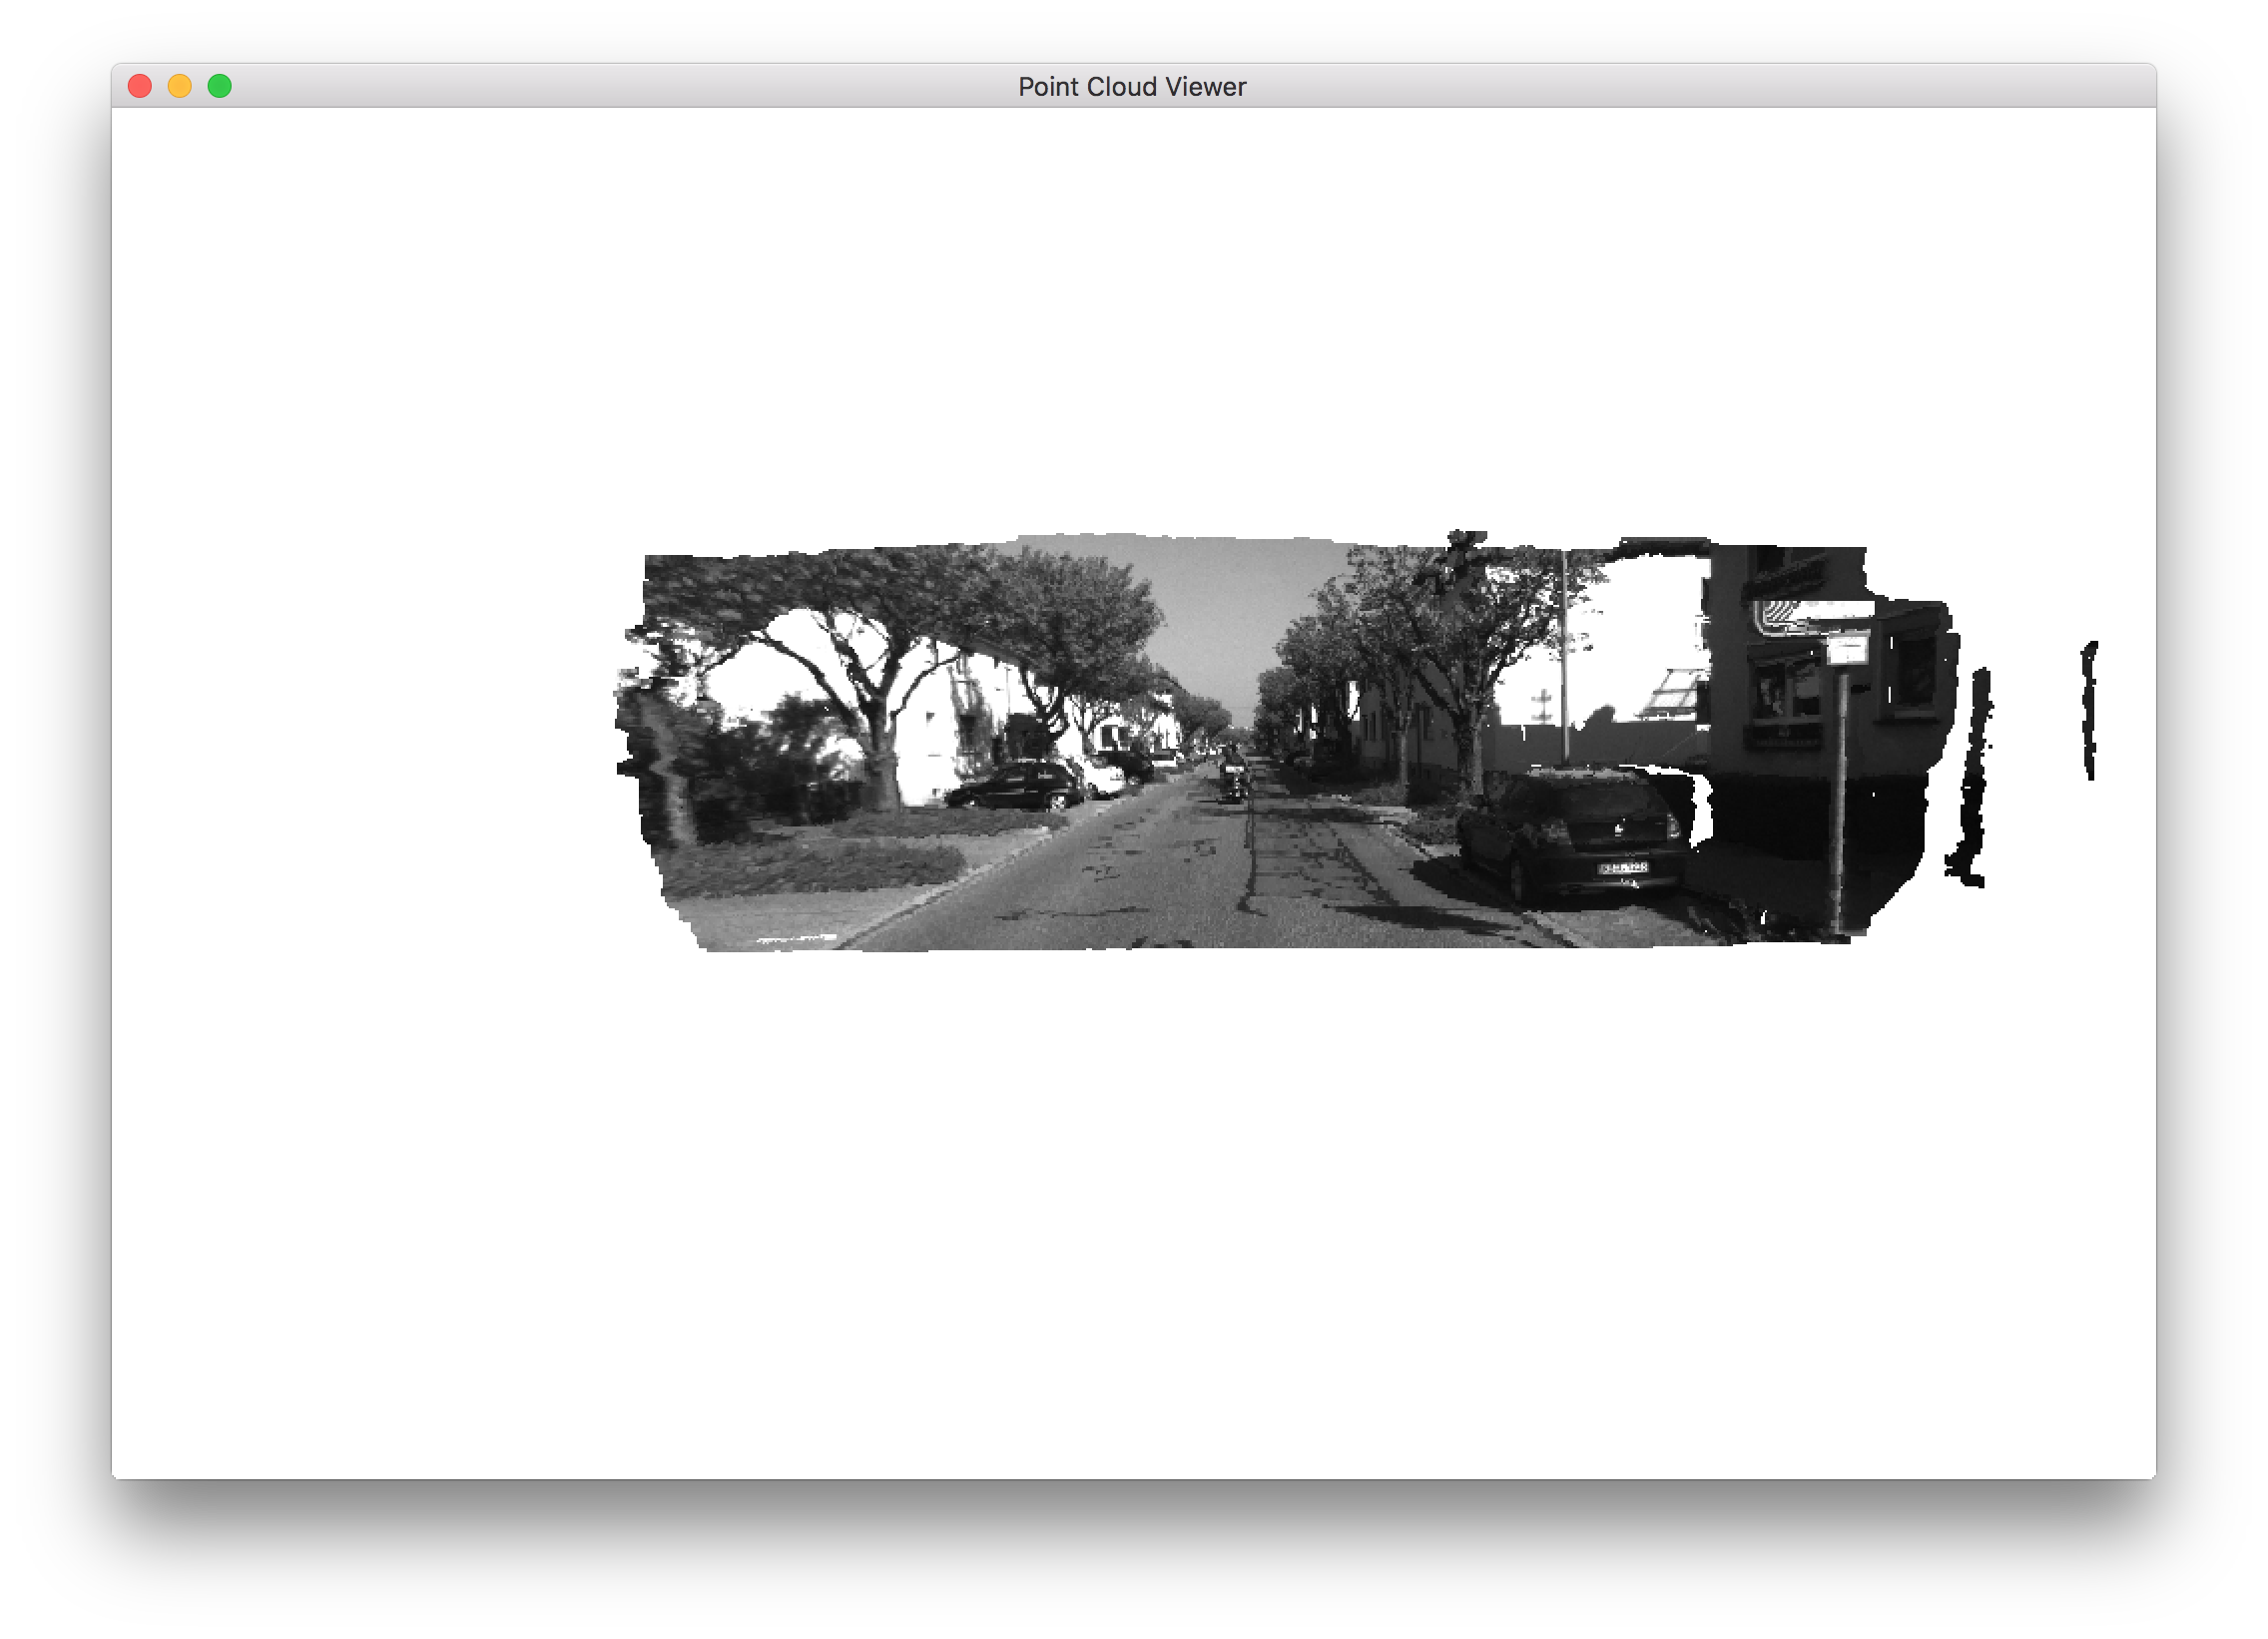
\includegraphics[height=6cm]{fig/disparity.png}
        \caption{Snapshot of \texttt{Pangolin} view of left-eye view as point cloud}
        \label{fig:disparity}
    \end{figure}

    \textsf{\textbf{Task 3}}
    The snapshot of point cloud view from RGB-D images is shown in Fig.~\ref{fig:build_map}.
    \begin{figure}[!h]
        \centering
        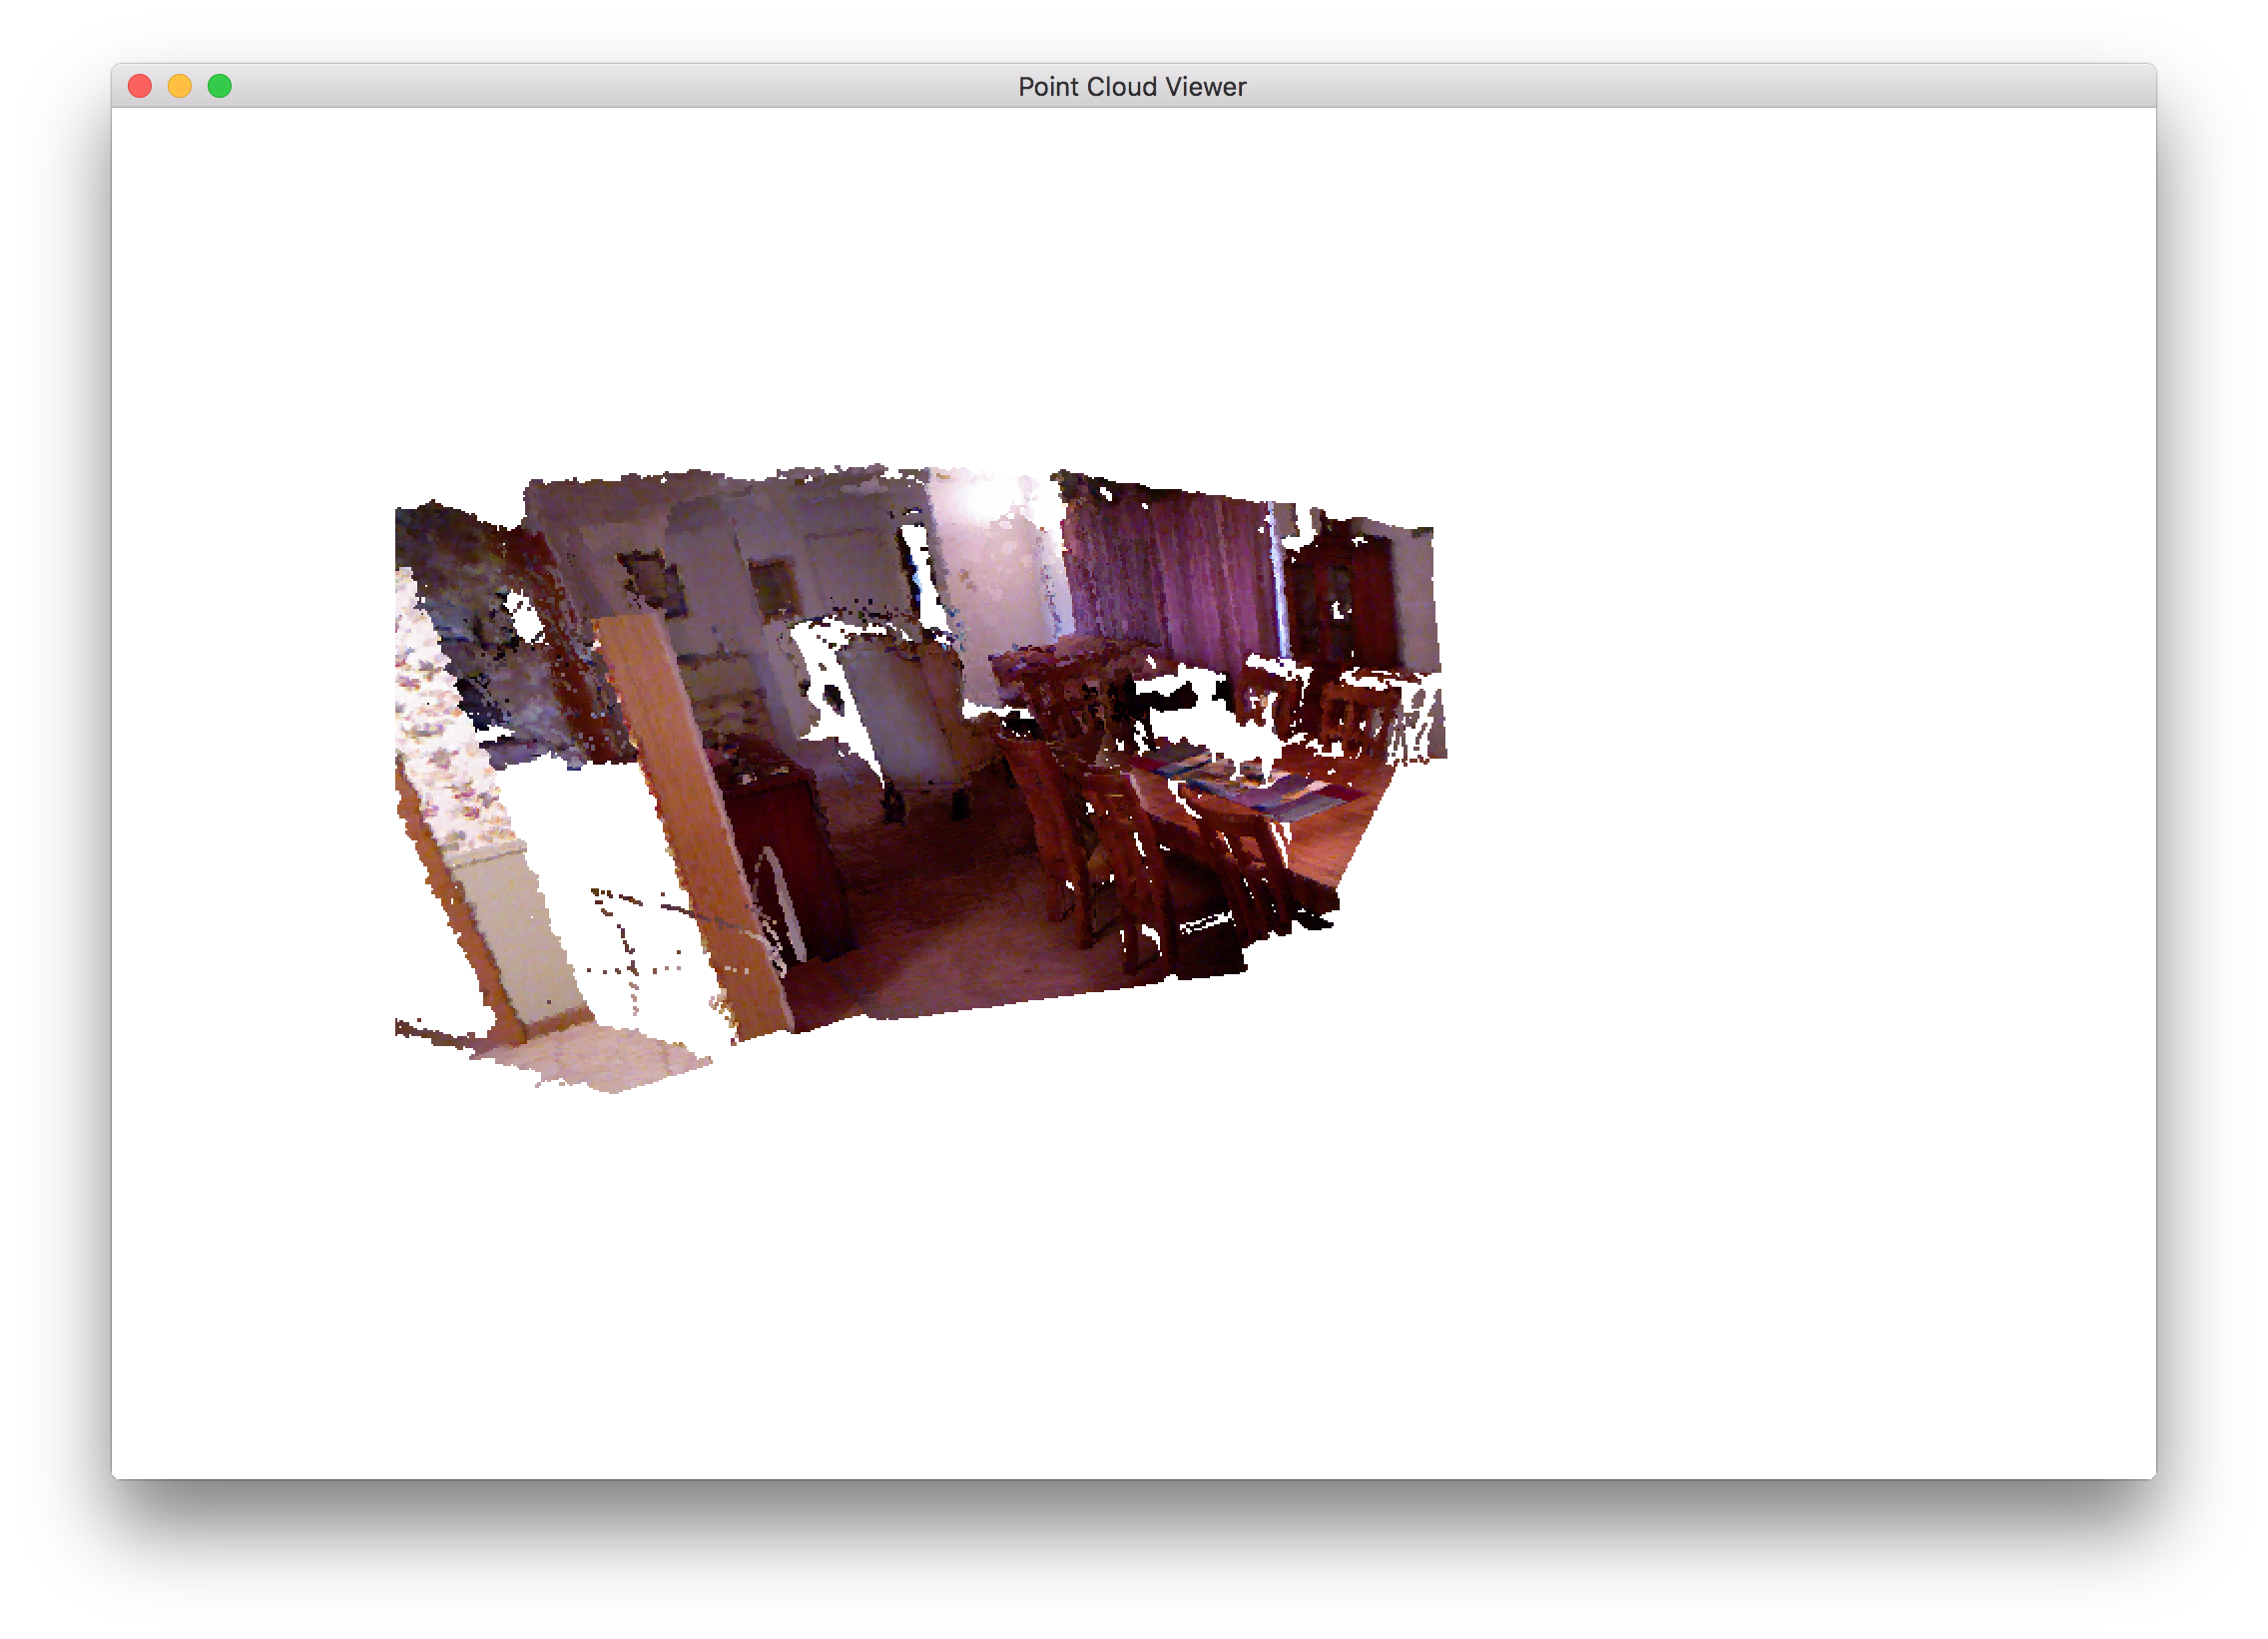
\includegraphics[height=6cm]{fig/build_map.png}
        \caption{Snapshot of \texttt{Pangolin} view of RGB-D images as point cloud}
        \label{fig:build_map}
    \end{figure}

    
\end{document}
